% Options for packages loaded elsewhere
\PassOptionsToPackage{unicode}{hyperref}
\PassOptionsToPackage{hyphens}{url}
%
\documentclass[
]{article}
\usepackage{amsmath,amssymb}
\usepackage{iftex}
\ifPDFTeX
  \usepackage[T1]{fontenc}
  \usepackage[utf8]{inputenc}
  \usepackage{textcomp} % provide euro and other symbols
\else % if luatex or xetex
  \usepackage{unicode-math} % this also loads fontspec
  \defaultfontfeatures{Scale=MatchLowercase}
  \defaultfontfeatures[\rmfamily]{Ligatures=TeX,Scale=1}
\fi
\usepackage{lmodern}
\ifPDFTeX\else
  % xetex/luatex font selection
\fi
% Use upquote if available, for straight quotes in verbatim environments
\IfFileExists{upquote.sty}{\usepackage{upquote}}{}
\IfFileExists{microtype.sty}{% use microtype if available
  \usepackage[]{microtype}
  \UseMicrotypeSet[protrusion]{basicmath} % disable protrusion for tt fonts
}{}
\makeatletter
\@ifundefined{KOMAClassName}{% if non-KOMA class
  \IfFileExists{parskip.sty}{%
    \usepackage{parskip}
  }{% else
    \setlength{\parindent}{0pt}
    \setlength{\parskip}{6pt plus 2pt minus 1pt}}
}{% if KOMA class
  \KOMAoptions{parskip=half}}
\makeatother
\usepackage{xcolor}
\usepackage[margin=1in]{geometry}
\usepackage{longtable,booktabs,array}
\usepackage{calc} % for calculating minipage widths
% Correct order of tables after \paragraph or \subparagraph
\usepackage{etoolbox}
\makeatletter
\patchcmd\longtable{\par}{\if@noskipsec\mbox{}\fi\par}{}{}
\makeatother
% Allow footnotes in longtable head/foot
\IfFileExists{footnotehyper.sty}{\usepackage{footnotehyper}}{\usepackage{footnote}}
\makesavenoteenv{longtable}
\usepackage{graphicx}
\makeatletter
\def\maxwidth{\ifdim\Gin@nat@width>\linewidth\linewidth\else\Gin@nat@width\fi}
\def\maxheight{\ifdim\Gin@nat@height>\textheight\textheight\else\Gin@nat@height\fi}
\makeatother
% Scale images if necessary, so that they will not overflow the page
% margins by default, and it is still possible to overwrite the defaults
% using explicit options in \includegraphics[width, height, ...]{}
\setkeys{Gin}{width=\maxwidth,height=\maxheight,keepaspectratio}
% Set default figure placement to htbp
\makeatletter
\def\fps@figure{htbp}
\makeatother
\setlength{\emergencystretch}{3em} % prevent overfull lines
\providecommand{\tightlist}{%
  \setlength{\itemsep}{0pt}\setlength{\parskip}{0pt}}
\setcounter{secnumdepth}{-\maxdimen} % remove section numbering
\newenvironment{cols}[1][]{}{}

\newenvironment{col}[1]{\begin{minipage}{#1}\ignorespaces}{%
\end{minipage}
\ifhmode\unskip\fi
\aftergroup\useignorespacesandallpars}

\def\useignorespacesandallpars#1\ignorespaces\fi{%
#1\fi\ignorespacesandallpars}

\makeatletter
\def\ignorespacesandallpars{%
  \@ifnextchar\par
    {\expandafter\ignorespacesandallpars\@gobble}%
    {}%
}
\makeatother
\usepackage{subfig}
\ifLuaTeX
  \usepackage{selnolig}  % disable illegal ligatures
\fi
\IfFileExists{bookmark.sty}{\usepackage{bookmark}}{\usepackage{hyperref}}
\IfFileExists{xurl.sty}{\usepackage{xurl}}{} % add URL line breaks if available
\urlstyle{same}
\hypersetup{
  pdftitle={Diamonds},
  pdfauthor={Oriade Simpson (s172084); Pietro Lombardo (s231756)},
  hidelinks,
  pdfcreator={LaTeX via pandoc}}

\title{Diamonds}
\usepackage{etoolbox}
\makeatletter
\providecommand{\subtitle}[1]{% add subtitle to \maketitle
  \apptocmd{\@title}{\par {\large #1 \par}}{}{}
}
\makeatother
\subtitle{02450 Introduction to Machine Learning \& Data Mining}
\author{Oriade Simpson (s172084) \and Pietro Lombardo (s231756)}
\date{From: 2023-09-05 To: 2023-10-03}

\begin{document}
\maketitle

\begin{center}
\includegraphics[width=0.4\linewidth]{Images/Universe2} \end{center}

\newpage
\newpage 
\newpage
\newpage 
\newpage
\newpage 
\newpage
\newpage
\newpage 
\newpage
\newpage 
\newpage
\newpage
\newpage
\newpage
\newpage
\newpage
\newpage

\hypertarget{contribution-table}{%
\section{Contribution Table}\label{contribution-table}}

\begin{center}\rule{0.5\linewidth}{0.5pt}\end{center}

\begin{longtable}[]{@{}lcc@{}}
\toprule\noalign{}
Task & Oriade & Pietro \\
\midrule\noalign{}
\endhead
\bottomrule\noalign{}
\endlastfoot
\textbf{Student ID} & s172084 & s231756 \\
------------- & -------------- & ------------- \\
Question 1 & x & \\
------------- & ------------- & ------------- \\
Question 2 & x & \\
------------- & ------------- & ------------- \\
Question 3 & & x \\
------------- & ------------- & ------------- \\
Question 4 & & x \\
------------- & ------------- & ------------- \\
Exam Prob 1 & & x \\
------------- & ------------- & ------------- \\
Exam Prob 2 & x & \\
------------- & ------------- & ------------- \\
Exam Prob 3 & x & \\
------------- & ------------- & ------------- \\
Exam Prob 4 & & x \\
------------- & ------------- & ------------- \\
Exam Prob 5 & & x \\
------------- & ------------- & ------------- \\
Exam Prob 6 & x & \\
\end{longtable}

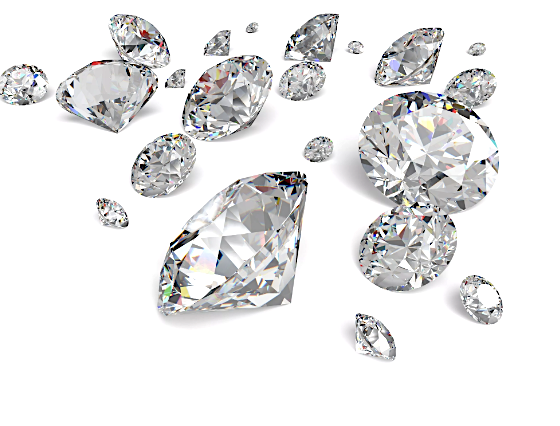
\includegraphics[width=0.3\linewidth]{Images/Diamond_Group}
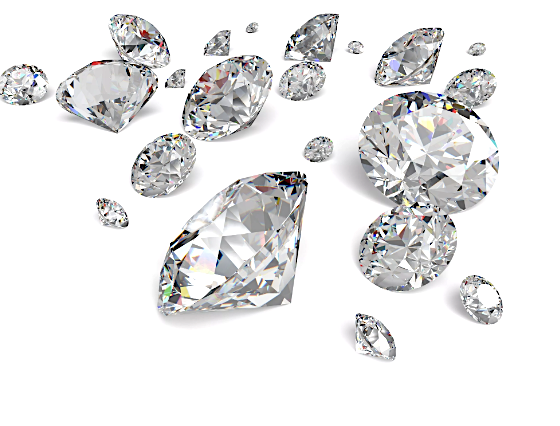
\includegraphics[width=0.3\linewidth]{Images/Diamond_Group}
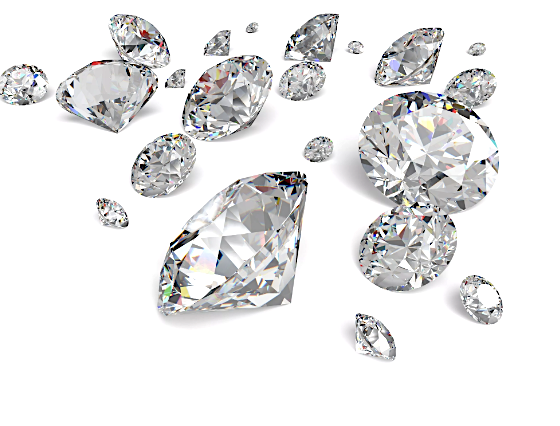
\includegraphics[width=0.3\linewidth]{Images/Diamond_Group}

\newpage

\hypertarget{question-1}{%
\section{Question 1}\label{question-1}}

\hypertarget{give-an-overview-and-introduction-to-the-dataset}{%
\subsubsection{Give an Overview and Introduction to the
Dataset}\label{give-an-overview-and-introduction-to-the-dataset}}

The International Diamond Grading System, created by The Gemological
Institute of America,focuses on the 4C's as a means to categorise
diamonds. The categories are explained on the Diamonds Search Engine,
which contains information about how loose diamonds are graded.

The Diamonds dataset used in this report is based on the Diamonds Search
Engine {[}1{]}.

The 4C's include :

\begin{itemize}
\tightlist
\item
  carat
\item
  cut
\item
  colour and
\item
  clarity.
\end{itemize}

The Diamonds dataset was obtained from the TidyVerse package developed
in R by Hadley Wickham and other contributors {[}4{]}.

The Diamonds dataset records 53,940 rows of diamonds and registers 10
attributes , including the 4C's.

Below, there is a brief overview about the variables in the dataset.

The length (\textbf{X}) , width (\textbf{Y}) and depth (\textbf{Z}) of
each diamond has been measured. The length ranges from 0 mm to 10.74 mm.
The width ranges from 0 mm to 58.9 mm and the depth ranges from 0 to
31.8 mm.

The carat of a diamond represents the weight of a diamond. The carat
ranges from 0.2 to 5.01 carats, where 1 carat is equal to 200 milligrams
(1/5 th of a gram).

The quality of the cut is categorised into fair, good, very good,
premium and ideal. The cut is an important feature because it determines
the sparkle and brilliance observed due to light refraction, which
potentially has an influence on the price.

The colour of a diamond is classified from D (best) to J (lowest). The
diamonds in group D are colourless. In the international diamond grading
system, colourless diamonds have the highest the grade. Diamonds that
are classified as J, often have a yellow tinge. One interesting factor
is the colour of the diamond, as many diamonds inside engagement rings
are G to J in colour. This colour is offset by a gold or silver band
{[}7{]}.

Clarity is categorised from IF to I1. IF is the best class. Here, F
means Flawless - without visible blemishes. Diamonds that contain
inclusions that are visible to the naked eye are given the worst class
of I1.\\
The last 3 variables or attributes of the dataset include the price, the
total depth percentage and the table.

The price of diamonds in US dollars ranges from \$326 to \$18,823 US
dollars. In the market, the price of diamonds may be based on the carat
weight.

The depth (total depth percentage) is a continuous variable which is the
total depth, from top to bottom of each diamond, divided by the mean
length and width.

The table is a continuous variable which is a measurement of the width
of the top of a diamond in relation to the widest point.

\hypertarget{what-is-the-overall-statement-of-interest}{%
\subsubsection{What is the Overall Statement of Interest
?}\label{what-is-the-overall-statement-of-interest}}

The idea is to analyse the dataset in order to determine relationships
between variables. More specifically, it may be interesting to discover
the relationship between two attributes: i.e.~the relationship between:

\begin{itemize}
\tightlist
\item
  The length and width of a colourless diamond
\item
  The colour and the table of the diamond
\item
  The carat and price of a colourless diamond
\item
  The carat and the table of a colourless diamond
\item
  The carat and the length of a colourless diamond
\item
  The carat and the width of a colourless diamond
\item
  The carat and the depth of a colourless diamond
\item
  The price corresponding to the cut of a diamond
\end{itemize}

\hypertarget{how-to-transform-data}{%
\subsubsection{How to Transform Data}\label{how-to-transform-data}}

Ideally the price could be determined in Danish Kroner, Pounds Sterling
or Euros, rather the US dollars. It may also be a good idea to transform
carats into milligrams to represent the weight of the diamond. The
attributes that are recorded in millimetres could also be converted to
centimetres.

\hypertarget{what-is-the-conclusion-of-previous-analysis}{%
\subsubsection{What is the Conclusion of previous
Analysis?}\label{what-is-the-conclusion-of-previous-analysis}}

In his R publication, Jon Ong has performed a brief analysis of this
dataset looking at the relationship between Cut vs.~Colour, Price
vs.~Cut, and Price vs.~Clarity. The results show that diamonds with a
Premium Cut have the highest carat {[}5{]}.

Poonam Rao has also performed a brief analysis of the diamonds dataset
where she performs data visualisation using scatterplots , histograms
and box-plots. She explains that diamonds that are categorised in the
Ideal group with regard to cut, often have a low weight {[}6{]} .

\hypertarget{what-do-you-aim-to-learn-from-the-data-using-classification-and-regression}{%
\subsubsection{What do you aim to learn from the data using
Classification and
Regression?}\label{what-do-you-aim-to-learn-from-the-data-using-classification-and-regression}}

A regression problem analyses the relationship between a dependent
variable and an independent variable. The Regression can be linear
regression or multiple linear regression.

It is possible to analyse the relationship between diamond length
(\textbf{X}) and diamond width (\textbf{Y}), the carat and the
depth(\textbf{Z}) in order to understand the relationship between these
variables. In the regression problem, we will predict the carat based on
the length, width and depth.

It is possible to look at the relationship between carat and price for 1
specific colour, cut and clarity of diamond in our regression problem.
One could observe the carat of the diamonds that are priced between
\$10,000 to \$20,000 USD.

A classification problem requires a dataset to be classified into two or
more categories. One idea is to choose the category of cut and determine
if the diamond is very good, premium cut or ideal cut? This can be done
using the diamond length (\textbf{X}) and diamond width (\textbf{Y}),
the carat and the depth(\textbf{Z}).

Another idea is to choose the category of colour and determine if the
diamond is D or J. This can be also be done using the diamond length
(\textbf{X}) and diamond width (\textbf{Y}), the carat and the depth(z).

It is also possible to choose the category of clarity and determine if
the diamond is IF , VS1 or I1 . This can be done using the diamond
length (\textbf{X}) and diamond width (\textbf{Y}), the carat and the
depth(\textbf{Z}).

\hypertarget{question-2}{%
\section{Question 2}\label{question-2}}

\hypertarget{describe-if-the-attributes-are-discretecontinuous-nominalordinalintervalratio}{%
\subsubsection{Describe if the attributes are discrete/continuous,
Nominal/Ordinal/Interval/Ratio}\label{describe-if-the-attributes-are-discretecontinuous-nominalordinalintervalratio}}

The table below shows the classification of the attributes. The cut,
colour, and clarity are ordinal factor variables. In the table below,
Cont. means continuous and Categ. means Categorical.

\hypertarget{attribute-table}{%
\subsection{Attribute Table}\label{attribute-table}}

\begin{longtable}[]{@{}
  >{\raggedright\arraybackslash}p{(\columnwidth - 20\tabcolsep) * \real{0.0730}}
  >{\centering\arraybackslash}p{(\columnwidth - 20\tabcolsep) * \real{0.0949}}
  >{\centering\arraybackslash}p{(\columnwidth - 20\tabcolsep) * \real{0.0949}}
  >{\centering\arraybackslash}p{(\columnwidth - 20\tabcolsep) * \real{0.0949}}
  >{\centering\arraybackslash}p{(\columnwidth - 20\tabcolsep) * \real{0.0949}}
  >{\centering\arraybackslash}p{(\columnwidth - 20\tabcolsep) * \real{0.0949}}
  >{\centering\arraybackslash}p{(\columnwidth - 20\tabcolsep) * \real{0.0949}}
  >{\centering\arraybackslash}p{(\columnwidth - 20\tabcolsep) * \real{0.0876}}
  >{\centering\arraybackslash}p{(\columnwidth - 20\tabcolsep) * \real{0.0949}}
  >{\centering\arraybackslash}p{(\columnwidth - 20\tabcolsep) * \real{0.0803}}
  >{\centering\arraybackslash}p{(\columnwidth - 20\tabcolsep) * \real{0.0949}}@{}}
\toprule\noalign{}
\begin{minipage}[b]{\linewidth}\raggedright
Attribute
\end{minipage} & \begin{minipage}[b]{\linewidth}\centering
Carat
\end{minipage} & \begin{minipage}[b]{\linewidth}\centering
Cut
\end{minipage} & \begin{minipage}[b]{\linewidth}\centering
Colour
\end{minipage} & \begin{minipage}[b]{\linewidth}\centering
Clarity.
\end{minipage} & \begin{minipage}[b]{\linewidth}\centering
Depth
\end{minipage} & \begin{minipage}[b]{\linewidth}\centering
Table
\end{minipage} & \begin{minipage}[b]{\linewidth}\centering
Price
\end{minipage} & \begin{minipage}[b]{\linewidth}\centering
Length (X)
\end{minipage} & \begin{minipage}[b]{\linewidth}\centering
Width(Y)
\end{minipage} & \begin{minipage}[b]{\linewidth}\centering
Depth (Z)
\end{minipage} \\
\midrule\noalign{}
\endhead
\bottomrule\noalign{}
\endlastfoot
Type & Cont. & Categ. & Categ. & Categ. & Cont. & Cont. & Discrete &
Cont. & Cont. & Cont. \\
Type & Ratio & Ordinal & Ordinal & Ordinal & Ratio & Ratio & Interval &
Ratio & Ratio & Ratio \\
\end{longtable}

There are no missing values or NAs in any column of the dataset. The
data is tidy from the TidyVerse. In the Premium cut group and Ideal cut
group of diamonds, there are some diamonds that have an outlying width,
which corresponds to the VS1 ad SI2 clarity groups.

\hypertarget{include-basic-summary-statistics-of-the-attributes-including-correlation}{%
\subsubsection{Include basic summary statistics of the attributes,
including
correlation}\label{include-basic-summary-statistics-of-the-attributes-including-correlation}}

There are many diamonds that have a carat between 0.2 and 1, with the
average carat being 0.7.\\
Therefore it may be interesting to narrow in on the dataset and only
look at diamonds that are between 1 and 5 carat, and exclude all
diamonds below 1 carat. The average length of a diamond (\textbf{X}) is
5.731 mm. It may be interesting to look at diamonds that are between 6
and 10 millimetres long.\\
The average price of a diamond in this dataset is \$3,932.8 USD. There
is a lower quantile of \$950 dollars and upper quantile of \$5,324.5
USD. It may be interesting to narrow down the price range and focus on
diamonds that are between \$326 - \$5000 USD. However \$5000 - \$15,000
USD or \$10,000 - £\$20,000 USD may also be suitable ranges to focus on.
Many of the diamonds have the average table of approximately 61.7.
Diamonds have an average depth of 3.5. It may be interesting to explore
diamonds that have a depth (\textbf{Z}) between 5 and 10. It may be
interesting to choose diamonds with a specific clarity, IF, SI2, VS1 and
narrow down on the cut to look at only 1 type of cut. There are 21,000
Ideal cut diamonds, which makes this the most common category. One could
choose the very good (12,082) , premium ( 13,791) or ideal cut diamonds
to focus on.

\hypertarget{summary-statistics-table}{%
\subsection{Summary Statistics Table}\label{summary-statistics-table}}

\begin{longtable}[]{@{}
  >{\raggedright\arraybackslash}p{(\columnwidth - 14\tabcolsep) * \real{0.1442}}
  >{\centering\arraybackslash}p{(\columnwidth - 14\tabcolsep) * \real{0.1154}}
  >{\centering\arraybackslash}p{(\columnwidth - 14\tabcolsep) * \real{0.1154}}
  >{\centering\arraybackslash}p{(\columnwidth - 14\tabcolsep) * \real{0.1635}}
  >{\centering\arraybackslash}p{(\columnwidth - 14\tabcolsep) * \real{0.1250}}
  >{\centering\arraybackslash}p{(\columnwidth - 14\tabcolsep) * \real{0.1250}}
  >{\centering\arraybackslash}p{(\columnwidth - 14\tabcolsep) * \real{0.0865}}
  >{\centering\arraybackslash}p{(\columnwidth - 14\tabcolsep) * \real{0.1250}}@{}}
\toprule\noalign{}
\begin{minipage}[b]{\linewidth}\raggedright
Variable
\end{minipage} & \begin{minipage}[b]{\linewidth}\centering
No.~Obs.
\end{minipage} & \begin{minipage}[b]{\linewidth}\centering
Mean
\end{minipage} & \begin{minipage}[b]{\linewidth}\centering
Variance
\end{minipage} & \begin{minipage}[b]{\linewidth}\centering
Standard Dev
\end{minipage} & \begin{minipage}[b]{\linewidth}\centering
Lower Quart
\end{minipage} & \begin{minipage}[b]{\linewidth}\centering
Median
\end{minipage} & \begin{minipage}[b]{\linewidth}\centering
Upper quart
\end{minipage} \\
\midrule\noalign{}
\endhead
\bottomrule\noalign{}
\endlastfoot
Carat. & 53,940 & 0.797 & 0.2247 & 0.474 & 0.4 & 0.7 & 1.04 \\
Cut. & 53,940 & & & & & & \\
Colour & 53,940 & & & & & & \\
Clarity & 53,940 & & & & & & \\
Total Depth \% & 53,940 & 61.749 & 2.052 & 1.433 & 61 & 61.8 & 62.5 \\
Table & 53,940 & 57.457 & 4.992 & 2.234 & 56 & 57.0 & 59.0 \\
Price & 53,940 & 3932.80 & 15915629 & 3989.44 & 22.59 & 24.69 & 27.64 \\
Length(X) & 53,940 & 5.731 & 1.258 & 1.122 & 4.71 & 5.70 & 6.54 \\
Width (Y) & 53,940 & 5.734 & 1.305 & 1.142 & 4.72 & 5.71 & 6.54 \\
Depth(Z) & 53,940 & 3.538 & 0.498 & 0.706 & 2.91 & 3.53 & 4.04 \\
\end{longtable}

\hypertarget{correlation-table}{%
\subsection{Correlation Table}\label{correlation-table}}

\begin{center}\rule{0.5\linewidth}{0.5pt}\end{center}

\begin{longtable}[]{@{}ll@{}}
\toprule\noalign{}
Correlation & Value \\
\midrule\noalign{}
\endhead
\bottomrule\noalign{}
\endlastfoot
X \& Y & 0.9747 \\
Y \& Z & 0.9520 \\
X \& Z & 0.9707 \\
carat \& X & 0.9750 \\
\end{longtable}

\begin{itemize}
\tightlist
\item
  There is a positive correlation between Length(\textbf{X}) and
  Width(\textbf{Y}).
\item
  There is a positive correlation between Width(\textbf{Y}) and
  Depth(\textbf{Z}).
\item
  There is a positive correlation between Length(\textbf{X}) and
  Depth(\textbf{Z}).
\item
  There is a positive correlation between carat and Length(\textbf{X})
\end{itemize}

\newpage

\hypertarget{data-visualization}{%
\section{3) Data visualization}\label{data-visualization}}

\hypertarget{representation-of-the-data-set}{%
\subsection{Representation of the data
set}\label{representation-of-the-data-set}}

The data set is composed by different type of data as discussed above.
In order to manage the ordinal attributes (\emph{cut}, \emph{color} and
\emph{clarity}), they can be converted into ordinal numbers (from 1 to
the upper level number) according to their ranking.

After the conversion, the data set appears as below:

\begin{longtable}[]{@{}rrrrrrrrrr@{}}
\caption{Head of the diamonds dataset arranged for the
PCA}\tabularnewline
\toprule\noalign{}
carat & cut & color & clarity & depth & table & price & x & y & z \\
\midrule\noalign{}
\endfirsthead
\toprule\noalign{}
carat & cut & color & clarity & depth & table & price & x & y & z \\
\midrule\noalign{}
\endhead
\bottomrule\noalign{}
\endlastfoot
0.23 & 5 & 2 & 2 & 61.5 & 55 & 326 & 3.95 & 3.98 & 2.43 \\
0.21 & 4 & 2 & 3 & 59.8 & 61 & 326 & 3.89 & 3.84 & 2.31 \\
0.23 & 2 & 2 & 5 & 56.9 & 65 & 327 & 4.05 & 4.07 & 2.31 \\
0.29 & 4 & 6 & 4 & 62.4 & 58 & 334 & 4.20 & 4.23 & 2.63 \\
0.31 & 2 & 7 & 2 & 63.3 & 58 & 335 & 4.34 & 4.35 & 2.75 \\
0.24 & 3 & 7 & 6 & 62.8 & 57 & 336 & 3.94 & 3.96 & 2.48 \\
\end{longtable}

\hypertarget{issues-with-outliers-in-the-data}{%
\subsubsection{Issues with outliers in the
data}\label{issues-with-outliers-in-the-data}}

To have a general idea of the distribution of the values assumed by the
attributes, a list of histograms can be displayed:

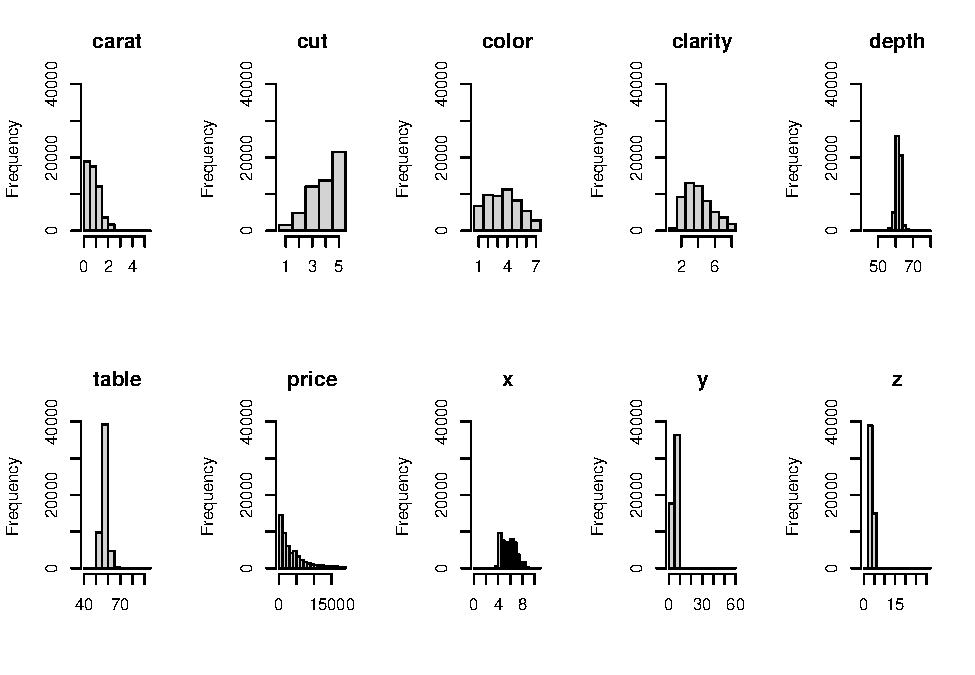
\includegraphics{Report_files/figure-latex/unnamed-chunk-4-1.pdf}

Some of the histograms seem to be affected by outliers in the data. It
can be seen by looking at the horizontal axis of each graph and by
noticing that bins do not cover all the axis values but only a limited
range. This is very evident in the attributes \emph{table} and in the
dimensions \emph{y} and \emph{z}. This attributes contain very extreme
values that wrongly set the axis limits. In order to detect them, the
data set can be sorted from the smallest value of a specific attribute
to the largest value of the same attribute. By doing so, it can be
selected the 99.99 percentile, which corresponds to the highest
observations of the data set sorted by one of the attributes. If the
values assumed by the attribute are not physical or are very different
from the other values, the specific observation can be discarded.

The \(99.99^{th}\) percentile of the data set sorted by the \emph{table}
shows the following data:

\begin{verbatim}
##       carat cut color clarity depth table price    x    y    z
## 24933  2.01   1     3       3  58.6    95 13387 8.32 8.31 4.87
## 50774  0.81   1     3       2  68.8    79  2301 5.26 5.20 3.58
## 51343  0.79   1     4       3  65.3    76  2362 5.52 5.13 3.35
\end{verbatim}

The first row has a value of \emph{table} very far from the other two
rows. It is very unlikely that, considering a data set of 53940
diamonds, there is a diamond with the \emph{table} 16 percentage points
bigger than the second-biggest \emph{table} diamond. For this reason,
the row nr. 24933 of the data set will be canceled.

As for the attribute \emph{y} (width), it can be followed the same
procedure by sorting the data set by the width and looking at the
\(99.99^{th}\) percentile:

\begin{verbatim}
##       carat cut color clarity depth table price     x     y    z
## 24068  2.00   4     5       2  58.9    57 12210  8.09 58.90 8.06
## 25999  4.01   4     6       1  61.0    61 15223 10.14 10.10 6.17
## 27416  5.01   1     7       1  65.5    59 18018 10.74 10.54 6.98
## 27631  4.50   1     7       1  65.8    58 18531 10.23 10.16 6.72
## 49190  0.51   5     2       5  61.8    55  2075  5.15 31.80 5.12
\end{verbatim}

It can be seen that the first and the last rows have very larger values
of \emph{y} with respect to the the other three rows belonging to the
\(99.99^{th}\) percentile. It is very unlikely that, considering such a
big number of diamonds, there are two diamonds with dimensions so
different from the others. So the two rows containing the two outliers
will be canceled

Finally, sorting the data set by the \emph{z}-dimension, the
\(99.99^{th}\) percentile is composed by the following records:

\begin{verbatim}
##       carat cut color clarity depth table price     x     y     z
## 23645  3.65   1     5       1  67.1  53.0 11668  9.53  9.48  6.38
## 24068  2.00   4     5       2  58.9  57.0 12210  8.09 58.90  8.06
## 27131  4.13   1     5       1  64.8  61.0 17329 10.00  9.85  6.43
## 27416  5.01   1     7       1  65.5  59.0 18018 10.74 10.54  6.98
## 27631  4.50   1     7       1  65.8  58.0 18531 10.23 10.16  6.72
## 48411  0.51   3     2       5  61.8  54.7  1970  5.12  5.15 31.80
\end{verbatim}

The last record has a value of \emph{z} very far from the other ones, so
it can be considered as an outlier and so it will be removed from the
data set.

\hypertarget{possible-distributions-followed-by-the-data}{%
\subsubsection{Possible distributions followed by the
data}\label{possible-distributions-followed-by-the-data}}

Now that the data set is free from outliers, the histograms of the
attributes will be more meaningful about the possible distribution the
data follow for each variable:

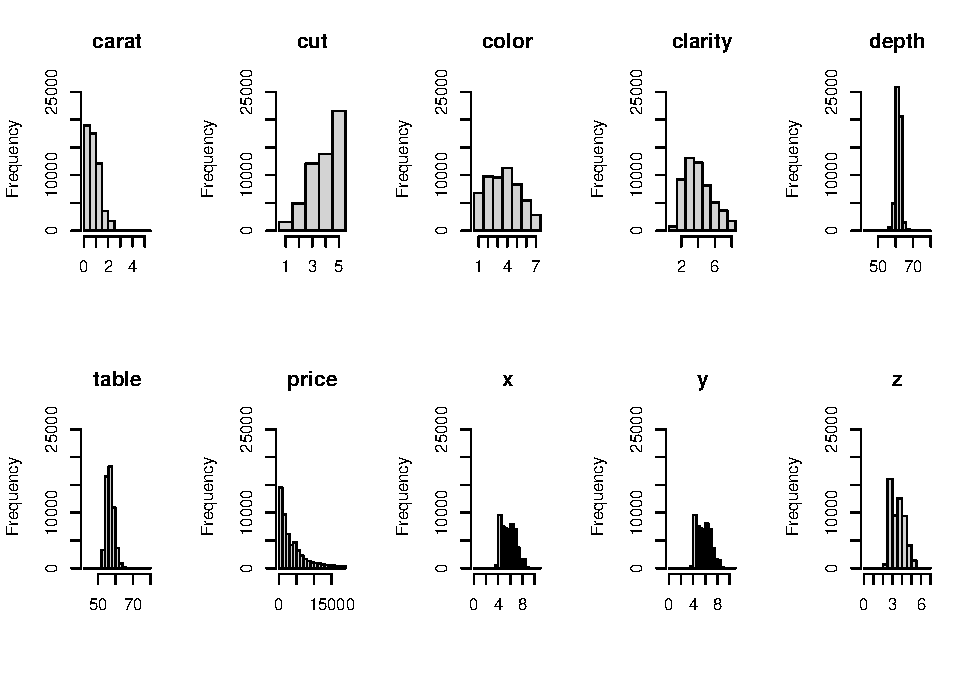
\includegraphics{Report_files/figure-latex/unnamed-chunk-8-1.pdf}

From the graphs, some considerations about the distribution of each
attribute can be listed: - attributes \emph{depth} and \emph{table}
appear to be normally distributed since they follow quite well the
gaussian bell curve and they are almost symmetric; - attributes
\emph{carat} and \emph{price} seem to follow an exponential
distribution, since each bin is smaller than the previous one and larger
than the following one; - attributes \emph{clarity}, \emph{x}, \emph{y}
and \emph{z} appear to follow a log-normal distribution, since they
follow a asymmetric bell curve with the sample-mode smaller than the
mean.

\hypertarget{correlation-of-variables}{%
\subsubsection{Correlation of
variables}\label{correlation-of-variables}}

Correlation between variables can be studied by producing the matrix of
scatter plots of each combination of two attributes against each other.
Scatter plots are not so meaningful with ordinal data (\emph{cut},
\emph{color} and \emph{clarity}), so they are removed from the data set
and points of the plots are colored according to the attribute
\emph{cut} in the attempt of finding some pattern of the data. The
matrix is shown below:

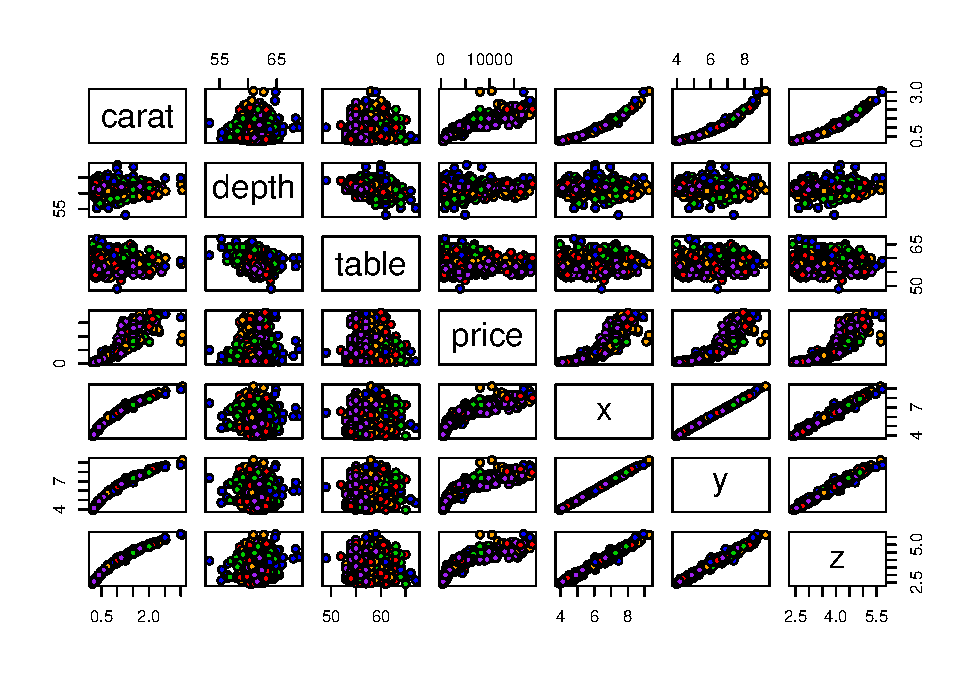
\includegraphics{Report_files/figure-latex/unnamed-chunk-9-1.pdf} The
plots confirm the very high correlation between the variables
\emph{carat}, \emph{x}, \emph{y} and \emph{z}, as already computed in
the Table 3. In addition, also the \emph{price} appears to be slightly
correlated with the variables \emph{carat}, \emph{x}, \emph{y} and
\emph{z}. The other variables do not show any specific pattern and also
the \emph{cut} does not seem to distinguish any cluster of the data.

\hypertarget{principal-component-analysis}{%
\subsection{Principal component
analysis}\label{principal-component-analysis}}

The aim of the Principal Component Analysis (``PCA'' from now on), is to
simplify the problem dimension by reducing the number of variables which
explains the behavior of the diamonds' price.

Below the standard deviations of the variables are shown:

\begin{verbatim}
##   carat     cut   color clarity   depth   table   price       x       y       z 
##    0.47    1.12    1.70    1.65    1.43    2.23 3989.44    1.12    1.14    0.71
\end{verbatim}

Since standard deviation of \emph{price} is some orders of magnitude
larger than the others, the dataset has to be standardized by
subtracting the mean and dividing by the standard deviation of the whole
set of observations of that variable.

\begin{cols}

\begin{col}{0.55\textwidth}
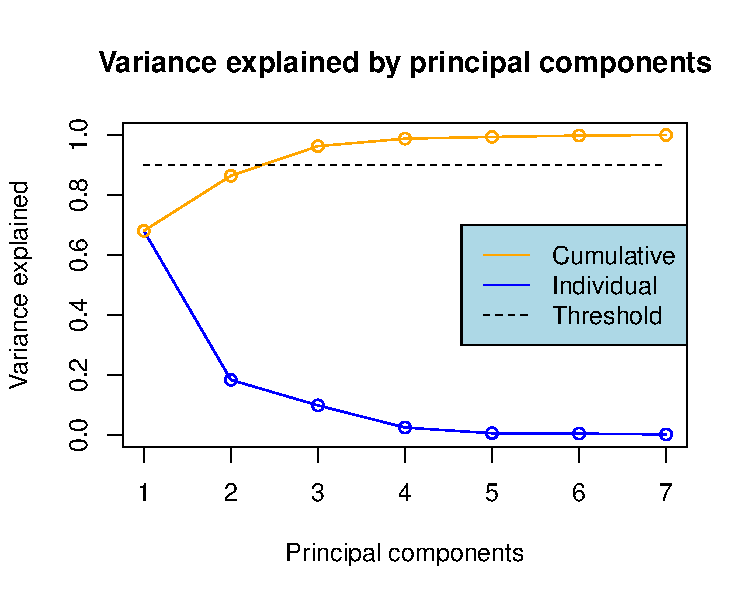
\includegraphics{Report_files/figure-latex/unnamed-chunk-12-1.pdf}

\end{col}

\begin{col}{0.05\textwidth}
~

\end{col}

\begin{col}{0.40\textwidth}
The new standardized dataset can be now used to perform the Singular
Value Decomposition (SVD), which gives rise to three different matrices:
\(U\), \(\Sigma\) and \(V^T\). By the extraction of the diagonal of the
matrix \(\Sigma\), it can be seen how much variance is explained by each
principal component. The cumulative explained variance should reach the
percentage of 90\% in order to describe properly the main features of
the dataset.

The figure on the left shows that the first 4 principal components
explain little less than the 90\% of variance

\end{col}

\end{cols}

\begin{cols}

\begin{col}{0.55\textwidth}
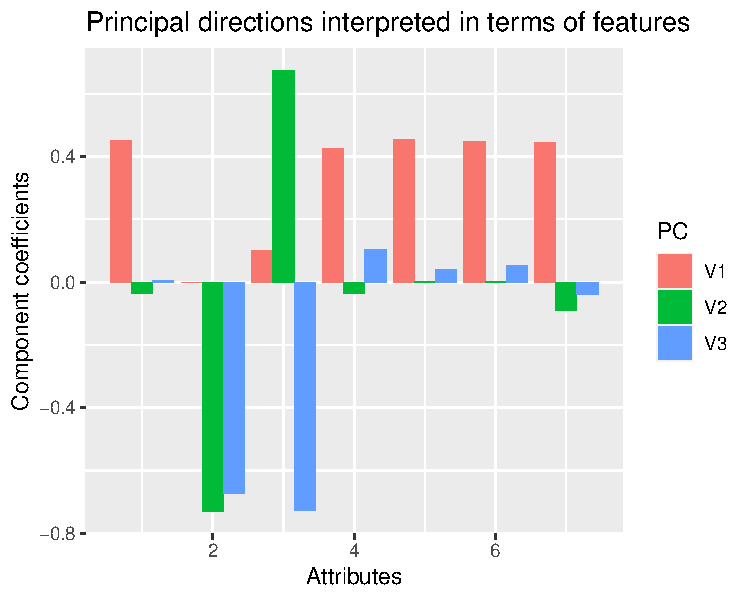
\includegraphics{Report_files/figure-latex/unnamed-chunk-13-1.pdf}

\end{col}

\begin{col}{0.05\textwidth}
~

\end{col}

\begin{col}{0.40\textwidth}
The matrix \(V^T\) contains the ten deca-dimensional vectors defining
the principal components (PCs). Focusing on the first four PCs, they
contains the weights associated to each of original component. The
figure on the left shows the valuea of the weights. It can be noticed
that the first PC mainly describes the dimensional quantities of the
diamonds (\emph{carat}, size in \emph{x}, \emph{y}, \emph{z}) and the
\emph{price}. It seems that these five characteristics alone explain
half of the variability of the diamonds. As for the second PC, it
focuses more on the quality characteristics (\emph{cut}, \emph{color},
\emph{clarity}) and on the \emph{table}.

\end{col}

\end{cols}

\begin{cols}

\begin{col}{0.55\textwidth}
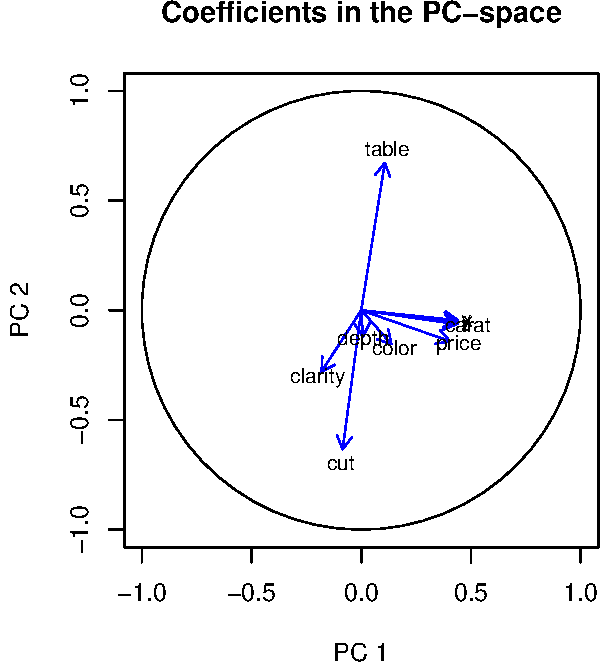
\includegraphics{Report_files/figure-latex/unnamed-chunk-14-1.pdf}

\end{col}

\begin{col}{0.05\textwidth}
~

\end{col}

\begin{col}{0.40\textwidth}
Unfortunately, it is impossible to represent data in a four-dimensional
space, so data are projected onto the bi-dimensional space defined by
the first two PCs. Coefficients can be projected in this space as well,
showing the directions followed by original attributes. It can clearly
be seen that the first PC is eastward oriented, so that it collects very
well the eastward attributes. Probably, the second PC is southward
directed so that it collects the southward attributes (with the plus
sign) and the northward \emph{table} attribute (with the minus sign)

\end{col}

\end{cols}

Data can be projected in all the possible bi-dimensional spaces defined
by each combination of two of the PCs. By projecting them, some
insteresting features can be observed, as shown by the four graphs
below.

\begin{itemize}
\tightlist
\item
  Variable \emph{cut} can assume five possible levels, so it is the
  easiest one to be visualized. The graph shows that \emph{cut} varies
  mostly in the direction of the second PC, so the \emph{cut} of
  diamonds strongly depends on their quality features (the better are
  \emph{color} and \emph{clarity}, the better will be the cut), and is
  less affected by the size (\emph{x}, \emph{y} and \emph{z}) and the
  \emph{carat} (weight);
\item
  variable \emph{price} is strongly asymmethrical towards low values,
  and it is very evident also in the graph where cold blue is
  predominant with respect to light blue. \emph{Price} strongly varies
  with the first PC, so it depends on quantity factors of diamonds (the
  bigger and heavier is the diamond, the more expensive will be) more
  than on quality ones;
\item
  variable \emph{carat} is very concentrated between 0 and 1 and
  widespread beyond 1. So, in order to have a better visualization, the
  graph below represent the logarithm of the \emph{carat}. It can be
  seen that it is correlated to the dimensional quantities explained by
  the first PC (the more expensive and bigger is the diamond, the
  heavier will be) more than quality ones;
\item
  variable \emph{color} has a better representation if data are
  projected onto the plan defined by the second and forth PCs. It can be
  seen that \emph{color} varies with the forth PC, so it is correlated
  with \emph{clarity}, \emph{cut} and \emph{table}.
\end{itemize}

\begin{center}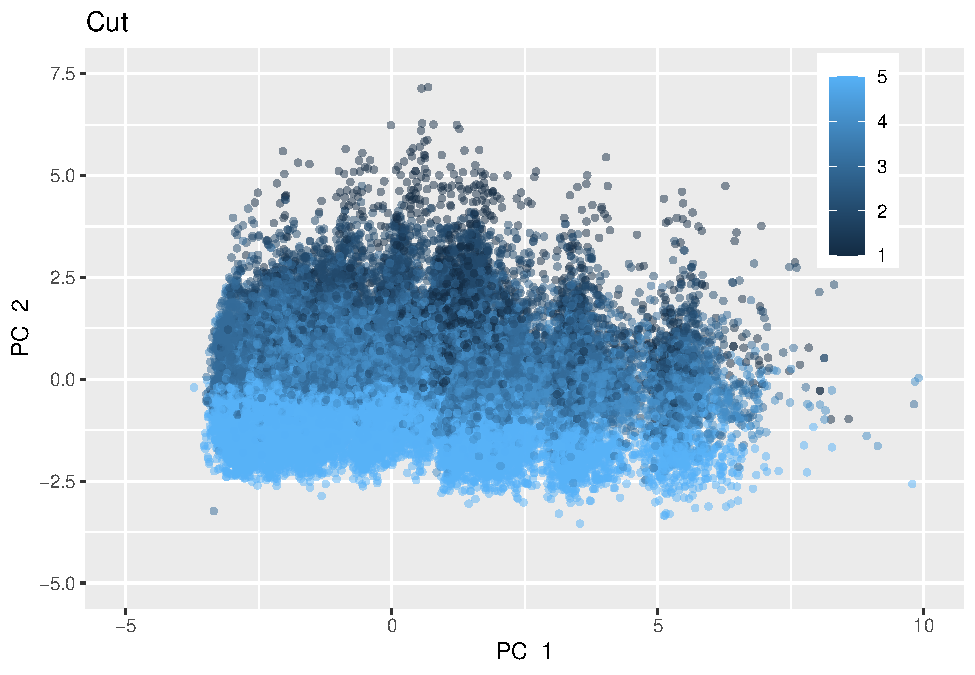
\includegraphics[width=0.75\linewidth]{Report_files/figure-latex/unnamed-chunk-15-1} \end{center}

\hypertarget{results-what-data-have-shown}{%
\section{4) Results: what data have
shown}\label{results-what-data-have-shown}}

\newpage

\hypertarget{exam-problems}{%
\section{Exam Problems}\label{exam-problems}}

\textbf{Question 1} \textbar{} Spring 2019 question 2 Which of the
following statements are true about the types of the attributes in the
Urban Traffic dataset?

Answer \textbf{B}: the attribute \(x_1\) is ordinal because it can be
said that time-interval number 5 is greater than the time-interval
number 4 since it is later in the day but it makes no sense to sum and
subtract them

\textbf{Question 2} \textbar{} Spring 2019 question 2 Consider again the
Urban Traffic dataset from table 1 and in particular the 14 and 18th
observation . Which of the following statements about the p-norm
distance dp (.,.) is correct ?

Answer \textbf{A}: The Maximum Norm Distance is 7.0

\textbf{Question 4} \textbar{} Spring 2019 question 2 Which one of the
following statements is true?

Answer \textbf{D}: PC2 has a negative coefficient multiplying \(x_1\),
so if an observation has a low value of \(x_1\) it means that the PC2
decreases very little for the contribution of \(x_1\). On the other
hand, PC2 has positive coefficients multiplying \(x_2\), \(x_3\) and
\(x_5\) so if an observation has a high value of them, it means that the
PC2 increases a lot thanks to their the contribution

\newpage

\hypertarget{references}{%
\section{References}\label{references}}

\begin{enumerate}
\def\labelenumi{\arabic{enumi})}
\item
  Grading Loose Diamonds, Diamonds Search Engine,
  ``\url{https://www.diamondse.info/diamonds-grading.asp}'', Accessed 22
  September 2023
\item
  Gemological Institute of America, Learn How a Diamond is Graded,
  (2009), YouTube ``\url{https://www.youtube.com/watch?v=oqhaty0ny0g}''
\item
  Diamond Prices Index,
  ``\url{https://www.diamondse.info/diamonds-price-index.asp}'' Accessed
  14 September 2023
\item
  Wickham H, Averick M, Bryan J, Chang W, McGowan LD, François R,
  Grolemund G, Hayes A, Henry L, Hester J, Kuhn M, Pedersen TL, Miller
  E, Bache SM, Müller K, Ooms J, Robinson D, Seidel DP, Spinu V,
  Takahashi K, Vaughan D, Wilke C, Woo K, Yutani H (2019). ``Welcome to
  the tidyverse.''~Journal of Open Source Software,~4(43),
  1686.~\url{doi:10.21105/joss.01686}
\item
  Jon Ong, Diamond Data Analysis , (2018),
  ``\url{https://rpubs.com/gokusun327/diamonddatatest}'' , Accessed 22
  September 2023
\item
  Poonam Rao , Exploratory Data Analytics, (2020),
  ``\url{https://medium.com/swlh/exploratory-data-analysis-21bbf3887e28}''
\item
  Paul Gian, Beyond 4C's - Real Insights to Buying Diamonds ,
  ``\url{https://beyond4cs.com/color/}'', Accessed 22 September 2023
\end{enumerate}

\end{document}
